\documentclass[12pt,a4paper]{amsart}
\usepackage{amsfonts}
\usepackage{amsthm}
\usepackage{amsmath}
\usepackage{amscd}
\usepackage[latin2]{inputenc}
\usepackage{t1enc}
\usepackage[mathscr]{eucal}
\usepackage{indentfirst}
\usepackage{graphicx}
\usepackage{graphics}
\usepackage{pict2e}
\usepackage{epic}
\numberwithin{equation}{section}
\usepackage[margin=2.9cm]{geometry}
\usepackage{epstopdf}
\usepackage{hyperref}

 \def\numset#1{{\\mathbb #1}}

 

\theoremstyle{plain}
\newtheorem{Th}{Theorem}[section]
\newtheorem{Lemma}[Th]{Lemma}
\newtheorem{Cor}[Th]{Corollary}
\newtheorem{Prop}[Th]{Proposition}

 \theoremstyle{definition}
\newtheorem{Def}[Th]{Definition}
\newtheorem{Conj}[Th]{Conjecture}
\newtheorem{Rem}[Th]{Remark}
\newtheorem{?}[Th]{Problem}
\newtheorem{Ex}[Th]{Example}

\newcommand{\im}{\operatorname{im}}
\newcommand{\Hom}{{\rm{Hom}}}
\newcommand{\diam}{{\rm{diam}}}
\newcommand{\ovl}{\overline}

\begin{document}
\title{Turing Mechanisms and Morphogenesis}
\author{Luke Mattfeld}
\address{Eastern Washington University \\ Department of Mathematics} 
\email{lukemattfeld@gmail.com}

\begin{abstract}
  The aim of this paper is to provide a brief overview and analysis of the conception of Morphogens according to Alan Turing in his paper
  On the Chemical Basis of Morphogenesis \cite{turing}, the nature of the behavior produced by the resulting equations,
  and some visual numerics demonstrating the patterns formed by varying reactions and initial constants.
\end{abstract}

\maketitle

\section{Introduction}

  The number of patterns in the world around us is quite remarkable
  There are numerous animals, plants, bacteria, etc
  which exhibit complex and seemingly pre-programmed patterns
  Yet the exact source and predictability of these patterns is mostly unknown
  This is what motivated Alan Turing to investigate and subsequently publish a paper \cite{turing} trying to determine what could cause these patterns; more specifically, what mathematical models, based on known and hypothesized biological interactions, could produce and predict patterns found in nature
  His paper deals specifically with patterns found in animal coats.

  At the time, the concept was far less researched than it is today, so Turing had far less data to go on and much more hypothesizing
  Yet, the models he came up with produce quite astounding results, and are still used as a base for research today.

  Turing began his model-building by simplifying things considerably
  Turing knew that the patterns observed in nature must be the result of a complex interaction between cells, chemicals, DNA, and other biomechanical processes
  But to begin with such a model would be nearly impossible
  Modeling the exact interaction of each system, as well as solving the resulting equation to test for the existence of patterns is a monumental task even today
  Turing figured that some abstraction could be done on these interactions, and that some simple mechanics could explain the majority of the phenomena observed.

  Turing knew this simplification would not explain everything
  In fact, he began his paper by saying, "This model will be a simplification and an idealization, and consequently a falsification."
  \cite{turing} What a great example of why mathematical models are valuable though they cannot tell the whole story.

\section{Morphogenesis and Turing Patterns}

  Turing hypothesized the existence of chemicals known as morphogens which would be responsible for the growth of specific cells
  Depending on the concentration of different morphogens in different regions, cells would grow accordingly
  These morphogens, being chemicals, would react with each other, and so the initial distribution of the morphogens would determine the final chemical balance of the system.

  However, chemical processes are typically stabilizing in nature and alone could not explain the unstable patterns observed
  Here is where Turing had a rather simple, though profound, insight
  These chemicals would also diffuse in space, similar to how heat diffuses
  Diffusion, another stabilizing process, would at first glance do nothing to cause the instabilities that formed patterns
  However, Turing found that given differing diffusion rates among morphogens, their concentrations would produce unstable equilibrium; you get patterns.

  A more grounded analogy (in understanding, not in reality) for what is taking place can be found in Murray's book on mathematical biology \cite{murray}
  Imagine a field of long tall grass
  If exposed to flame, eventually the entire field will burn; the fire in any location will "react" with nearby dried grass, catching it on fire, and so on through the entire field.

  Now, let us imagine the field is spotted with a number of grasshoppers
  But not just any grasshoppers; these grasshoppers sweat
  Profusely
  While this is humorous, it is necessary for the analogy
  Imagine these grasshoppers can sweat to the extent that the surrounding grass becomes damp
  This time, when the field combusts, as the fire reaches the grasshoppers they begin to sweat, and at the same time move away from the fire
  As long as they can travel faster than the fire, they will leave a trail of damp grass behind them that will not burn
  So, you will be left with a field that is all burned, except with some patches containing sweaty grasshoppers.

  This leaves us with an interaction of short-range activation and long-range inhibition; The fire activates more fire in the nearby grass, but at a longer distance, it is causing the grasshoppers to sweat and inevitably hampering its own spread
  This concept of short-range activation and long-range inhibition is a general principle in the study of pattern formation
  It extends into the field of mechanics of cells and neurotransmission in the brain.

  Now, before we continue there are a few caveats Turing came up with
  From the analogy of the grasshoppers and the fire, on can imagine that the end results of the field burn varies greatly on a number of factors; The rate at which the fire spreads, the rate at which the grasshoppers move, the number of grasshoppers, and the rate at which the grasshoppers sweat all play a critical role in describing the interaction
  In some cases, the fire may be so much quicker than the grasshoppers that the entire field will burn regardless
  Conversely, if there are a considerable number of grasshoppers, they sweat a great deal, and they move constantly, the fire may only affect a small portion of the field.

  These variables are analogous to the amounts, diffusion rates, and reaction types of morphogens
  Consequently, only certain setups will produce patterns
  According to Turing, six systems would form steady states (fig 1.1)
  And out of these six, only one forms Turing patterns (fig 1.2) \cite{kondo}

  \begin{align*}
  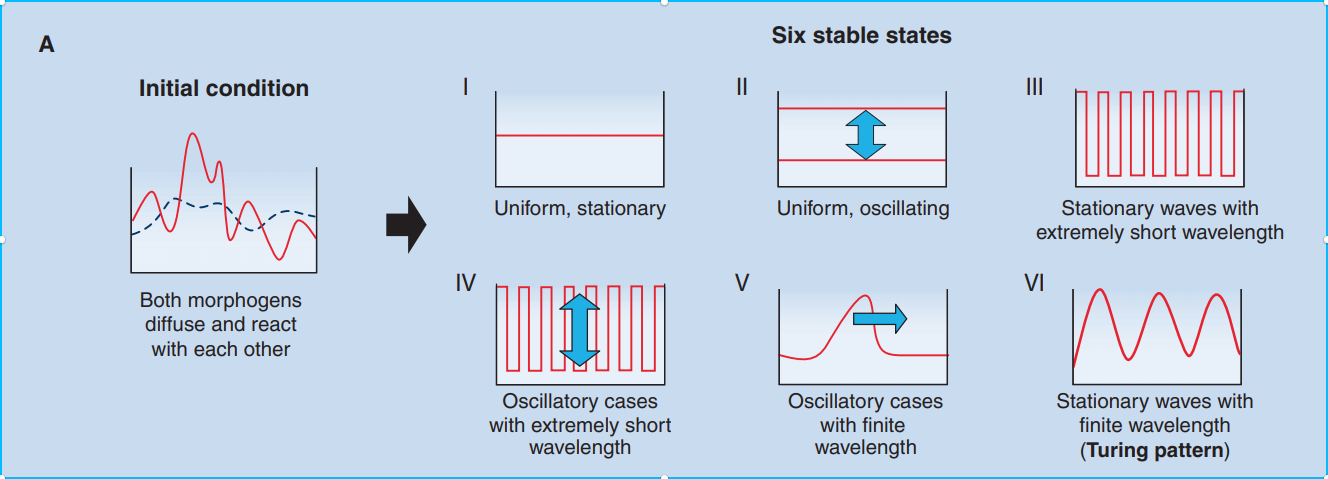
\includegraphics[width=0.75\textwidth]{stable_states.png}\\
  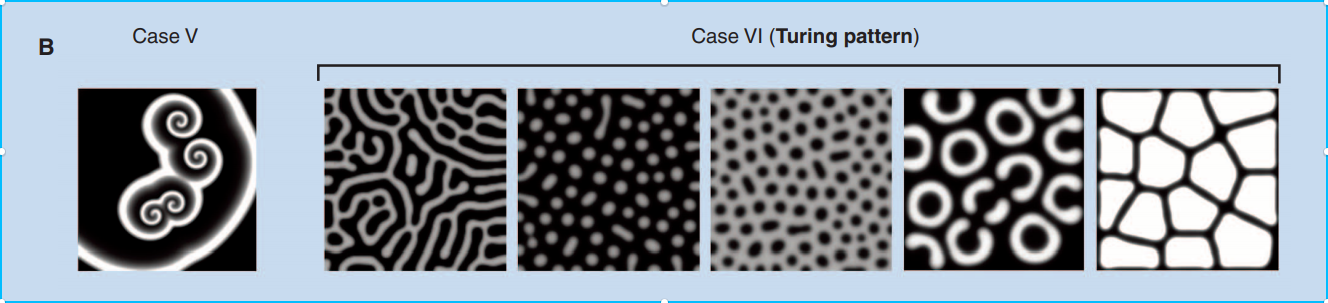
\includegraphics[width=0.75\textwidth]{turing_pattern.png}
  \end{align*}

  Another caveat is that in a system of complete symmetry, these reactions would not take place to form patterns
  There must be some asymmetric "kick-off" for the process to begin
  In the real world, these are rather easy to come by due to the sheer number of random events and variables at the conception of such a system.


\section{Reaction Diffusion}

As stated before, the model Turing came up with was one of chemical reaction and diffusion of morphogens.
The general equation for such a model, called the Reaction Diffusion Equation is shown below:
\\
\textbf{General Reaction-Diffusion equation:}
\begin{align*}
  \frac{\partial A}{\partial t} = F(A,B) + D_{A} \nabla A \\
  \frac{\partial B}{\partial t} = G(A,B) + D_{B} \nabla B
\end{align*}

Here, A and B are the concentration of two chemical morphogens.

$F(A,B)$ describes the reaction of A and B according to $A$

$G(A,B)$ describes the reaction of B and A according to $B$

$D_{A} and D_{B}$ describe the diffusion rate of each chemical, respectively

$\nabla^2 A$ and $\nabla^2 B$ Describe the change in each chemical with respect to space (aka, diffusion).

This equation describes how the concentration of each changes over time (thus, it's in the form of a Differantial Equation).
Here, the chemical rections are abstracted out, and for any real model will be replaced with one related to the chemicals at play.

A fairly common model is the Gray-Scott model, which sets:

$$F(A,B)=-AB^2+f(1-A)$$
$$G(A,B)=AB^2-(k+f)B$$

Where f is the rate at which A is beeing added - "feed", k is the rate at which B is being removed - "kill"

\section{Numerics}
We can see some patterns resulting from variations on the Gray Scott model of chemical reaction.
Samples can be found in (./Numerics/Samples).
The code to produce such images (and to produce realtime formation based on initial and boundry conditions)
is included in this submission (./Numerics/diffusion.cu)


\newpage
\begin{thebibliography}{99} 

\bibitem{turing} Alan M Turing: \textit{On the Chemical Basis of Morphogenesis}, \begin{verbatim} http://www.dna.caltech.edu/courses/cs191/paperscs191/turing.pdf
\end{verbatim}

\bibitem{murray} J.D. Murray: \textit{Mathematical Biology Vol. II}, \begin{verbatim} http://pcleon.if.ufrgs.br/pub/listas-sistdin/MurrayII.pdf
\end{verbatim}

\bibitem{maini} Prof. Philip Maini: \textit{Turing's Theory of Developmental Pattern Formation}, \begin{verbatim} https://www.youtube.com/watch?v=pN8tVldm6QY
\end{verbatim}

\bibitem{kondo} Shigeru Kondo and Takashi Miura: \textit{Reaction-Diffusion Model as a Framework for Understanding Biological Pattern Formation}, \begin{verbatim} https://science.sciencemag.org/content/329/5999/1616
\end{verbatim}

\bibitem{ctrain} The Coding Train: \textit{Reaction Diffusion Algoritm in P5.JS}, \begin{verbatim} https://thecodingtrain.com/CodingChallenges/013-reactiondiffusion-p5.html
\end{verbatim}

\bibitem{sims} Karl Sims: \textit{A simulation of two virtual chemicals reacting and diffusing on a 2D grid using the Gray-Scott model}, \begin{verbatim} http://karlsims.com/rd.html
\end{verbatim}

\end{thebibliography}


\vspace*{\fill}
\end{document}